\chapter{Identity and Trajectory Construction}

%123456789 123456789 123456789 123456789 123456789 123456789 123456789 123456789

In this chapter we discuss actual techniques to group the \glspl{det} into
desired clusters, i.e. creating \glspl{iden} as per \autoref{ssec:task}.
We show how we combine visual information of the image
(\autoref{ch:features}) with metadata to provide \glspl{iden}.

\section{Trajectories}

In this section, we focus on grouping \glspl{det} together without the use of visual information, i.e. purely based on the metadata. In other words we create trajectories as per \autoref{sec:workflow}. By its nature the \glspl{det} within a single trajectory are from consecutive frames and physically close together, displaying one moving object.

The reason for this step is to group the \glspl{det} together in cases
where the visual information --- which processing may be complicated --- is not
needed. The trajectories then serve as a ``building blocks'' for subsequent
processes.


% The trajectories serve as a ``building blocks'' for more
% complicated \glspl{iden}. Due to the way they are constructed the trajectories
% are clusters of \glspl{det} that are physically close together. They are usually
% just list of \glspl{det} from the consecutive frames with just a minor changes
% in position of tracked object in-between the frames.

\subsection{Detection Metadata}

Let us briefly recall available metadata for each \gls{det} as introduced in
\autoref{ssec:input}:

\begin{itemize}
    \item $(x_0, x_1, y_0, y_1)$ -- Position of the bounding box of the detection given by $x$-coordinate of the left and the right edge and the $y$-coordinate of top and bottom edge respectively.
    \item Class of the \gls{det}, e.g. person, car or truck
    \item Identificator of a the camera
    \item Timestamp
\end{itemize}

\todo[inline=true]{\LaTeX{} Globalne zmensit mezery mezi ``items'' v ``itemize'' na neco lepsiho}

Let us start with a simplification. For now, we consider metadata of just two \glspl{det} at hand, and we explore if we can find out whether the \glspl{det} display the same object (i.e. in this context whether they belong to the same trajectory). We discuss each part of the metadata separately.

For each metadata we use a separate condition or set of conditions. We conclude that the \glspl{det} show the same object if all the condition are true. In some cases we show the simple condition in enough (\autoref{ssec:nonspatial_merging}). In other cases we derive additional values and then each of these values we compare with suitable threshold that needs to be find by experimenting with various settings (we discuss this topic further in \autoref{ssec:spatial_merging}).

Note that, even if some of the conditions for a given pair of \glspl{det} are not fulfilled, we can assign the \glspl{det} to the same trajectory later using transitivity. We elaborate further on this topic in \autoref{ssec:trajectory_generation}.

\subsection{Direct Conditions on Metadata}

\label{ssec:nonspatial_merging}

Let us start with the class of the \gls{det}. The class
gives us the most straight-forward conclusion.
If the two \glspl{det} at hand are of different classes we know for sure
that they can not display the same
object.\footnote{There a is quite
odd case where this seemingly obvious conclusion can be argued against. That
is, for example, when a person enters a car. Based on the actual definition of
the \gls{iden} we may consider it the same displayed object. As these cases
raises multiple questions (e.g. what should happen when multiple people enter the same vehicle), we shall consider a person entering the vehicle and the vehicle itself as different
\glspl{iden} and we leave further research in this topic for a
future work.} As a corollary, we therefore assume that the two \glspl{det} are
of the same class while investigating the rest of the metadata.

We can incorporate camera identificator just as easily. If the two
\glspl{det} are from different cameras, we do not explore the remaining
metadata, as they do not hold any useful information in such
case.\footnote{There
are approaches that assume that the two given cameras capture largely the same
area and are calibrated (for example \cite{hu2006principal}). However, we
assume no prior calibration and therefore we leave similar approaches for other
work} For example even if there is one detection in top left corner of one
camera, and in the exact same time there is another detection in top left corner
of another camera at the same time, we can not say if the \glspl{det}
display the same person or not. This is
because we do not know if the area within top left corner is the same as the
area in the top left corner of the second camera. In such case we have to use
a priori assumption and assign them to two different
trajectories.\footnote{Unless we have any additional information the a priori
assumption that two \glspl{det} belong to different golden \glspl{iden} (and thus also a trajectory) is more
likely to be true than the opposite. This holds at least under the assumption that there is no
golden \gls{iden} that would be represented by more than a half of the
\glspl{det} within given \gls{ses}.}

For an assignment into the same trajectory we therefore consider only \glspl{det}
from the same camera. We only elaborate on such cases in the remainder
of this subsection. We regard cases how to discover the same object across
different cameras later in this chapter (\autoref{sec:generating_identities}).

Lastly, let us consider additional information that we gain by using the timestamp.
In combination with the spatial data the timestamp can be helpful. However as
we mentioned in the introduction of this section
we are now interested in creating short trajectories (i.e. clusters of
\glspl{det} that are physically close together). Therefore
our approach to temporal information is simple: If the time difference is
bigger than selected threshold (say 1 second, however we experiment with
various settings), we assign the \glspl{det} to different trajectories. In the
opposite case we shall further evaluate secondary conditions on the spatial
information.

\subsection{Conditioning on spatial information}

\label{ssec:spatial_merging}

Now, let us focus on the last part of the metadata --- position of the bounding box within the frame. While the conditions we presented so far was simple, we propose more complex conditions for processing spatial information.

In order to sufficiently capture the information regarding the position let us first derive a few auxiliary quantities. When processing this spatial information we compare the selected auxiliary quantities with suitable thresholds. We find suitable subset of auxiliary quantities and threshold by empirical testing in \autoref{ch:evaluation}.

For brevity in the following lines we shall use height ($h = y_1 - y_0$) and
width ($w = x_1 - x_0$) of a \gls{det}'s bounding box.

\subsubsection{Displacement of Detections}

One of the quantities to consider when comparing two \glspl{det} is
their displacement. We shall compute the displacement with respect to centers
of the \glspl{det}. Formally we can compute a displacement as follows
(superscripts represent the \glspl{det} --- (A) or (B):

\begin{align*}
    c^{(A)} &= \left(\frac{x_0^{(A)} + x_1^{(A)}}{2}, \frac{y_0^{(A)} + y_1^{(A)}}{2}\right) &\vspace{1cm}&\text{center of detection }(A)\\
    c^{(B)} &= \left(\frac{x_0^{(B)} + x_1^{(B)}}{2}, \frac{y_0^{(B)} + y_1^{(B)}}{2}\right) &\vspace{1cm}&\text{center of detection }(B)\\
    d &= \delta_{euclid}(c^{(A)}, c^{(B)})&\vspace{1cm}&\text{displacement of the detections}
\end{align*}

\subsubsection{Relative Displacement}

However, such simple displacement only expresses the displacement within the screen of the camera. Now, we would like to take the perspective into the account.

If an object close to the camera moves, this movement translates to a larger displacement compared to the displacement caused by the object further from the camera. We propose to estimate the ``closeness'' to the camera without a prior calibration. We use the size of the bounding box of the detection to obtain approximation for distance from the camera (i.e. bigger the bounding box, more likely it is that the object is closer to the camera). This works well under the assumption that the objects are of similar sizes (i.e. all are people).

While this estimation is quite vague, it has additional advantages. For example it penalizes more the displacement of smaller objects. This means that we see the big movements of an adult (with big bounding box) more likely than the same movement of a child (with small bounding box).

Overall, this leads us to the definition of relative displacement where we divide the displacement by an average edge length of the bounding boxes:

$$\frac{d}{\left(h^{(A)} + w^{(A)} + h^{(B)} + w^{(B)}\right) / 4}$$

\subsubsection{Intersection over Union}

The last quantity we shall consider is so-called \gls{iou}. \Gls{iou} represents the ratio of the area covered by both bounding boxes (intersection) and the area covered by either of the bounding boxes (union). For a visual interpretation see \autoref{fig:iou}. Formally we can define the quantity for our rectangular bounding boxes as:

\begin{align*}
    \text{InterWidth} &= \min\left(x_1^{(A)}, x_1^{(B)}\right) - \max\left(x_0^{(A)}, x_0^{(B)}\right) \\
    \text{InterHeight} &= \min\left(y_1^{(A)}, y_1^{(B)}\right) - \max\left(y_0^{(A)}, y_0^{(B)}\right) \\
    \text{Intersection} &= \begin{cases}\text{InterWidth} \cdot \text{InterHeight} & \text{if InterWidth} > 0 \land \text{InterHeight} > 0 \\ 0 & \text{else}\end{cases} \\
    \text{Union} &= w^{(A)} h^{(A)} + w^{(B)} h^{(B)} - \text{Intersection} \\
    \text{IoU} &= \frac{\text{Intersection}}{\text{Union}}
\end{align*}

\begin{figure}
    \centering
    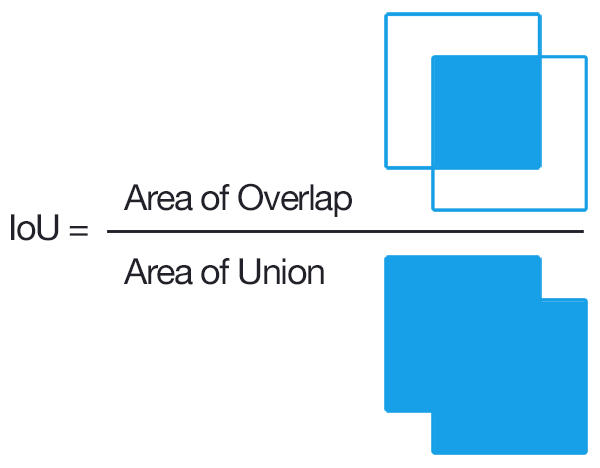
\includegraphics[width=6cm]{img/Intersection_over_Union_-_visual_equation.png}
    \caption[Visualization of Intersection over Union]{Visualization of Intersection over Union\\Source: Intersection over Union -- visual equation\protect\footnotemark{} by Adrian Rosebrock, CC BY-SA 4.0,\footnotemark{} via Wikimedia Commons}
    \label{fig:iou}
\end{figure}
\addtocounter{footnote}{-2}
\stepcounter{footnote}\footnotetext{\url{https://commons.wikimedia.org/wiki/File:Intersection_over_Union_-_visual_equation.png}}
\stepcounter{footnote}\footnotetext{\url{https://creativecommons.org/licenses/by-sa/4.0}}


\subsection{Trajectory generation}

\label{ssec:trajectory_generation}

So far we worked with only two \glspl{det} at the same time and derived a set of conditions. In this section we aim make a use of a context of the whole \gls{ses}. We further show how we generate the actual trajectories.

Firstly, let us note that we can not apply the conditions from \autoref{ssec:nonspatial_merging} and \autoref{ssec:spatial_merging} to every pair of \glspl{det} for practical reasons. Comparing every \gls{det} with every other \gls{det} takes quadratic time with respect to number of \glspl{det} and for hundreds of thousands of \glspl{det} is unfeasible to compute on standard hardware. Therefore, we need to lower the number of comparisons.

In order to do so we leverage the way we use timestamp as described in \autoref{ssec:nonspatial_merging}. We consider only \glspl{det} whose difference in timestamps are below a selected threshold. This means that we need to compare only pairs of \glspl{det} that fit within selected ``sliding time window''. We process the \glspl{det} in order of their timestamp.

When we process a new \gls{det} we add it to the sliding window. At the same time we remove all the \glspl{det} from the sliding window that are older than the timestamp of the new detection minus the threshold. Then we compare the new \gls{det} with all the \glspl{det} within the window. Using the sliding window dramatically decreases the number of comparison needed.

However, this approach does not limit the length of the single trajectory by selected threshold. We use ``transitive'' information about the trajectory. Namely, if a \gls{det} ($A$) belongs to the same trajectory as \gls{det} ($B$) and \gls{det} ($B$) belongs to same trajectory as \gls{det} ($C$), we can conclude that the \gls{det} ($A$) and \gls{det} ($C$) is of the same trajectory.

This process of finding if there is a transitive link between the two \glspl{det} may also pose a limitation on the number of \glspl{det} we can process effectively. To improve the performance in this regard we use standard Union-find architecture originally described by \cite{galler1964improved}. The architecture allows us to track which \glspl{det} belongs to which trajectory and merge them in almost constant\footnote{The actual complexity of the operation is inverse Ackermann function of the size of the structure per query (amortized) as were proved by \cite{tarjan1984worst}. For the details of the structure please refer to the attached code or the original research.} time per request.

Finally, let us note this approach of using transitive link is not only efficient but also have additional advantage. Let us consider a case where a person crosses entire view of a camera. Without this transitive connection we would need to set huge thresholds to match the first and last \gls{det} of this person (which would produce trajectories of poor quality). However, by using transitivity over other \glspl{det} we can match the first a last \gls{det} together ``through'' the \glspl{det} of the same person on the frame in between while keeping the thresholds low.

The overall approach for trajectory generation described in this subsection is summarized by \autoref{alg:trajectory_generation}.

\begin{algorithm}
 \SetKwData{Traj}{Trajectories}
 \SetKwData{Win}{SlidingWindow}
 \SetKwData{Det}{Detection}
 \SetKwData{ProcDet}{ProcessedDetection}
 \SetKwFunction{UnionFind}{UnionFind}
 \SetKwFunction{Queue}{Queue}
 \SetKwFunction{Top}{Top}
 \SetKwFunction{Ts}{Timestamp}
 \SetKwFunction{Pop}{Pop}
 \SetKwFunction{Add}{Add}
 \SetKwFunction{AddNs}{AddNewSet}
 \SetKwFunction{Union}{Union}
 \SetKwInOut{Input}{input}
 \SetKwInOut{Output}{output}

 \Input{List $X$ of detections sorted by timestamp, threshold $t$}
 \Output{List of generated trajectories (each trajectory as list of detections)}
 
 \BlankLine
 \Traj $\leftarrow$ \UnionFind{ }\;
 \Win $\leftarrow$ \Queue{ }\;
 \For{\Det $\in X$}{
  \While{\Det.\Ts $-$ \Win.\Top.\Ts $> t$} {
   \Win.\Pop{}\;
  }
  \Win.\Add{\Det}\;
  \Traj.\AddNs{\Det}\;
  \For{\ProcDet $\in$ \Win}{
   \If{All conditions for merging are met}{
    \Traj.\Union{\ProcDet, \Det}\;
   }
  }
 }
 \Return \Traj

 \caption{Trajectory Generation}
 \label{alg:trajectory_generation}
\end{algorithm}

\section{Identities}

\label{sec:generating_identities}

So far we have looked into how to cluster the \glspl{det} purely based on the metadata (i.e. how to create trajectories). Now we add the visual information (in form of feature vectors from \autoref{ch:features}) to also identify the same object in \glspl{det} that are physically far apart or captured by different cameras -- something that was not possible using just metadata. In other words we are interested in creating the \glspl{iden}. Each \gls{iden} then represents all the \glspl{det} of a single object. To find the correct \glspl{iden} is the final goal of our algorithm, and of this thesis.

\subsection{Trajectory Merging}

The first approach we evaluate directly works with trajectories generated in previous section. We consider trajectories as ``building blocks'' and merge them together into the \glspl{iden} by incorporating the visual information.

We base the merging of the trajectories on the distance between the \glspl{det} (or more, precisely, corresponding feature vectors) from the trajectories. We explore multiple distance functions (Euclidean, Manhattan, Cosine -- for definitions please refer to \autoref{sec:distances}) and their effect on the quality of resulting \glspl{iden}.

The straight-forward approach would be to consider each pair of trajectories and to compare each \gls{det} from one trajectory to each \gls{det} from the other trajectory. If the distance between the corresponding feature vectors is lower than selected threshold, we merge the trajectories together. This is quite similar to merging \glspl{det} into trajectories as described in previous section. However, it shares the same disadvantage -- the total number of comparison needed in quadratic in terms of number of \glspl{det}. In the previous case we solved this problem by using sliding window. If we use the sliding window here we lose the ability to merge trajectories with significant ``time gaps''. Therefore, we show another approach to decrease the number of comparison needed.


\subsubsection{Selection of Representants}

%We present a relatively simple approach to decrease number of comparison needed.

The idea behind the approach is to select from each trajectory a set of representants. We want to select a suitable set of representants that will preserve as much information as possible needed for creating appropriate \glspl{iden}. We then compare just pairs of representants instead of all pairs of \glspl{det}. As we show, if the representants are chosen well, the resulting \glspl{iden} will be nearly as good as if we were to compare all the pairs of \glspl{det}.

To show how to pick suitable representants, let us consider following case. Let there be a trajectory and let us pick two \glspl{det} from the trajectory that are similar in terms of their feature vectors. Now consider additional trajectory and one arbitrary \gls{det} from this trajectory in particular. The situation is shown in \autoref{fig:triangular}. The question we focus on is whether we should merge these trajectories together based on the three selected \glspl{det} or not. The straight-forward way to do it would be to compare the \gls{det} from the second trajectory to both of the \glspl{det} from the first trajectory. Note due to the triangular inequality as the two \glspl{det} from the first trajectory are similar, the two computed distances from the third \gls{det} should be similar too. Therefore, if we make our decision regarding the merging the trajectories based on just one of the two distances, we (in most cases) make just as good decision as if we computed both distances. Note that this observation relies on the triangular inequality and therefore holds only if the distance function used is a metric.

\begin{figure}
    \centering
    \def\svgwidth{\columnwidth}
    \scalebox{0.6}{\input{img/triangular.pdf_tex}}
    \caption[Usage of triangular inequality for the selection of representants]{Usage of the triangular inequality for the selection of representants. From the triangular inequality the distances $d_1$ and $d_2$ differs at most by the value of $d_s$, i.e. $\abs{d_1 - d_2} \leq d_s$}
    \label{fig:triangular}
\end{figure}

This leads us to the idea that for each trajectory from each set of similar \gls{det} we set only one of them as a representant. To be more precise for each trajectory we set a set of representants such that for each \gls{det} within the trajectory there is at least one representant, for which the distance to the detection is at most some threshold $\Delta_{rep}$. Refer to \autoref{alg:representants} to how to select such representants.

\begin{algorithm}
 \SetKwInOut{Input}{input}
 \SetKwInOut{Output}{output}

 \Input{Trajectory $T$ (as a list of feature vectors of detections), Threshold $\Delta_{rep}$}
 \Output{List of feature vectors of representants}
 
 \BlankLine
 $R \leftarrow$ \emph{empty list}\;
 \For(\tcp*[h]{outer loop}){$D_{new} \in T$}{
  \For{$D_{rep} \in R$}{
   \If{$\delta(D_{new}, D_{rep}) \leq \Delta_{rep}$}{
    skip to the next iteration of outer loop\;
   }
  }
  append $D_{new}$ to $R$\;
 }
 \Return $R$
 \caption{Selection of representants of a trajectory}
 \label{alg:representants}
\end{algorithm}

In context of many trajectories and detection this approach indeed gives some guarantees. Let us assume that we get a set of trajectories and we find set of representants by \autoref{alg:representants} with threshold $\Delta_{rep}$ for each trajectory. After selection of representants we merge the trajectories that have any representants closer than merging threshold $\Delta_{mrg}$.

If there is unknown partitioning (golden \glspl{iden}) that are ``well-separated'' in a certain sense by the distance function then we will obtain exactly this unknown golden partitioning. By the term ``well-separated'' we mean that the minimal distance between \glspl{det} from two distinct golden \glspl{iden} is at least $\Delta_{mrg}$ and that for each pair of \glspl{det} from the same golden \gls{iden} there exists path over \glspl{det} such that each subsequent \glspl{det} are at most $(\Delta_{mrg} - 2\Delta_{rep})$ apart. To visualize this situation see \autoref{fig:claim}. We formalize this claim:

% We can apply this observation in a context of more than just three \glspl{det}.
% Let us assume that we  start with trajectories that are ``clean'' (i.e.
% trajectory contain \glspl{det} of just a single golden \gls{iden}). Further
% assume that the golden \glspl{iden} are ``well-separated'' using the selected
% metric function in a following sense: The minimal distance between two
% \glspl{det} from different golden \glspl{iden} is at least $\Delta_{mrg}$
% and for every pair of \glspl{det} from any \gls{iden} there exists a sequence
% of \glspl{det} such that every \gls{det} is from the same \gls{iden} and
% and distance between two consecutive \glspl{det} is at most
% $\Delta_{mrg} - 2\Delta_{rep}$. Then the produced \glspl{iden} produced by
% selection representants by \autoref{alg:representants} and then merging
% trajectories that have \glspl{det} closer than $\Delta_{mrg}$
% are always exactly golden \glspl{iden}.


% The observation that will help us select proper representative is that if
% there are two \glspl{det} within a trajectory, that are similar (in terms of
% distance between their feature vectors), than whatever third \gls{det} is
% similar to the first \gls{det} is similar also to second \gls{det} (at least
% as long as we use metric and not generic distance as we show in a while).
% Therefore if there is a pair of similar \glspl{det} in a trajectory, we select
% at most one as a representant and discard the other. For systematic way of
% selecting representant leveraging this property see \autoref{alg:representants}.




% Our intuitive observation, that we need to preserve only one of the two similar
% \glspl{det} in a trajectory can be formalized as:

%This claim can be formalized as follows:

\begin{figure}
    \centering
    \def\svgwidth{\columnwidth}
    \input{img/claim.pdf_tex}
    \caption[Visualization of claim \ref{clm:claim}]{Visualization of claim \ref{clm:claim}. The figure shows two \glspl{iden}, first of them divided into three trajectories, latter into two. The Dots represents \glspl{det}, the black ones mark the representants. Solid lines (shown only is the first trajectory) connect \glspl{det} to the closes representant, these lines are at most $\Delta_{rep}$ long. Dashed lines connect representants themselves and thus are at longer than $\Delta_{rep}$. Dotted lines connect \glspl{det} of different trajectory but the same \gls{iden} (only a few are shown). The gray lines connect \glspl{det} of different \glspl{iden}.
    
    The claim considers situation where all ``gray distances'' are at least $\Delta_{mrg}$ and where we can walk from any \gls{det} of one \gls{iden} to another \gls{det} from the same \gls{iden} only by using the lines within the trajectories and the dotted lines that are at most $(\Delta_{mrg} - 2\Delta_{rep})$ long. In such cases the produces \glspl{iden} perfectly match the golden \glspl{iden} shown in the figure.}
    \label{fig:claim}
\end{figure}

\begin{claim}
\label{clm:claim}
Let:

\setlength{\itemsep}{0pt}
\setlength{\parskip}{0pt}

\begin{itemize}
    \item $D$ be a set of \glspl{det}
    \item $A$ a partitioning of $D$ (this represents golden \glspl{iden})
    \item $T$ partitioning of $D$ such that $(\forall t \in T) (\exists a \in A) (t \subseteq a)$ (this represents input ``clean'' trajectories)
    \item $\Delta_{rep}, \Delta_{mrg} \in \R^+$ such that $\Delta_{rep} < \Delta_{mrg}$
    \item $\delta$ be an metric function over $D$
    \item $r$ be a function $r: \Pt{D} \goto \Pt{D}$ such that $(\forall c \subseteq D) (\forall b \in c) (\exists b' \in r(c)) (\delta(b, b') \leq \Delta_{rep})))$ (this represents selection of representants obtained for example via \autoref{alg:representants})
    \item $\circ$ be a relation over $T$ such that $t\circ t' \Leftrightarrow (\exists d \in r(t)) (\exists d' \in r(t')) (\delta(d, d') \leq \Delta_{mrg})$ (two trajectories are in relation $\circ$ if we can merge them together)
    \item $\bullet$ be a transitive closure of $\circ$ (i.e. $t \bullet t' \Leftrightarrow (\exists n \in \N) (\exists (t_1, \ldots, t_n) \in T^n) (t = t_1 \land t' = t_n \land (\forall i) (t_i\circ t_{i+1}))$ (this relation is equivalence that represents final \glspl{iden} -- two trajectories are in relation $\bullet$ if and only if they were merged together)
\end{itemize}

If the following holds (i.e. the golden \glspl{iden} are ``well-separated''):
\begin{itemize}
    \item $(\forall a \in A)(\forall d, d' \in a) (\exists n \in \N) (\exists (d_1, \ldots, d_n) \in D^n) (d = d_1 \land d' = d_n \land (\forall i) (\delta(d_i, d_{i+1}) \leq \Delta_{mrg} - 2\Delta_{rep}))$
    \item $(\forall a, a' \in A) (\forall d \in a) (\forall d' \in a') (a \neq a' \Rightarrow \delta(d, d') > \Delta_{mrg})$
\end{itemize}

Then: $t\bullet t' \Leftrightarrow (\exists a \in A) (t \cup t' \subseteq a)$ (i.e. produced \glspl{iden} exactly match golden \glspl{iden})

% Let $D$ be a set of \glspl{det}, $A$ its partitioning, $\delta$ a metric over
% $D$, $T$ another partitioning of $D$ such that $(\forall t \in T) (\exists a \in A) (t \subseteq a)$ and thresholds $x_{rep}, x_{merge} \in \R^+$. Denote $r: \Pt{D} \goto \Pt{D}$ generator representants as per \autoref{alg:representants} with threshold $x_{rep}$. Now consider $R$ to be a relation over $T$ such that $tRt' \Leftrightarrow (\exists d \in r(t)) (\exists d' \in r(t')) (\delta(d, d') \leq x_{merge})$ and let $\widehat{R}$ be its transitive closure.

% If $\min_{a, a' \in A : a \neq a'} \min_{d \in a, d' \in a'} \delta(d, d') > x_{merge}$ and
% $(\forall a \in A)(\forall d, d' \in a)(\exists (d = d_1, d_2, \ldots, d_n = d') \subseteq a)(\forall i)(\delta(d_i, d_{i+1}) \leq x_{merge} - 2x_{rep})$ 
% then $t\widehat{R}t' \Leftrightarrow (\exists a \in A)(t \cup t' \subseteq a)$.

\end{claim}

% This claim basically tells us that if we start with the trajectories that
% are ``clean'' (i.e. each trajectory is a subset of some golden \gls{iden}) and
% the \glspl{iden} are well-separated (i.e. distance between golden \glspl{iden}
% are at least $x_{merge}$ and for any pair of the \glspl{det} within a \gls{iden}
% there is a sequence of \glspl{det} such thateach subseqent pair of \glspl{det} within the sequence is distant at most $(x_{merge} - 2x_{rep})$ and the ends
% of the sequence are the original two \glspl{det}, then the produced clustering
% of the \glspl{det} corresponds to the desired golden \glspl{iden}.

\begin{myproof}
First, let us prove that $t \bullet t' \Rightarrow (\exists a \in A) (t \cup t' \subseteq a)$. We shall prove this by contradiction, i.e. for now we assume
that $(\exists a \in A) (t \in a)$ and $(\exists a' \in A) (t' \in a')$ and $a \neq a'$. From property of $\bullet$ we know there is a sequence of $t_1, t_2, \ldots t_n$ (for some $n$), such that $(\forall i) (t_i \circ t_{i+1})$. Let
us take minimal $i$ such that $t_i$ and $t_{i+1}$ is not subset of the same
$a \in A$ (such $i$ exists as $t$ and $t'$ does belong to different $a$s).
For such $i$ (since $t_i \circ t_{i+1}$) there is $d \in t_i$ and
$d' \in t_{i+1}$ such that $\delta(d, d') \leq x_{mrg}$. However since $d \in a$
and $d' \in a'$ (such that $a \neq a'$) this is in contradiction with second
of the original assumptions.

Now let us prove that $(\exists a \in A) (t \cup t' \subseteq a) \Rightarrow t \bullet t'$. Let us choose $d \in t$ and $d' \in t'$ arbitrarily. By the
assumptions for elements of $a$ there is sequence $(d_0, \ldots, d_n) \in A^n$
such that $d = d_0 \land d' = d_n \land (\forall i) (\delta(d_i, d_{i+1}) \leq x_{mrg} - 2x_{rep}$. Now let us denote for each $i$ $t_i \in T$ such that
$d_i \in t_i$. Finally, let us denote $r_i = \mathrm{argmin}_{d \in r(t_i)} \delta(d, d_i)$. If $t_i = t_{i+1}$ then $t_i \circ t_{i+1}$ by definition.
So let us consider cases where $t_i \neq t_{i+1}$. In such case we can bound
the distance between $r_i$ and $r_{i+1}$ due to the triangle inequality:
$\delta(r_i, r_{i+1}) \leq \delta(r_i, d_i) + \delta(d_i, d_{i+1}) + \delta(d_{i+1}, r_{i+1}) \leq x_{rep} + (x_{mrg} - 2x_{rep}) + x_{rep} = x_{mrg}$. And as $r_i \in r(t_i)$ we can conclude that $(\forall i) (t_i \circ t_{i+1})$. Therefore $t \bullet t'$.\end{myproof}


\begin{cor}
If the distance between two closest \glspl{det} from different golden
\glspl{iden} is $\Delta_{between}$ and the distance between two most distance detection
of the same golden \gls{iden} is $\Delta_{within} < \Delta_{between}$, then for any set of ``clean''
trajectories (i.e. if each trajectory contains \glspl{det} only from single
golden \gls{iden}) the \autoref{alg:representants} for representant selection
with threshold $(\Delta_{between} - \Delta_{within} - \varepsilon) / 2$ (for arbitrarily small
$\varepsilon \in \R^+$) followed by merging based on representants with
threshold $\Delta_{between} - \varepsilon$ produces the golden \glspl{iden}.
\end{cor}

Let us note that the original assumption is fulfilled if the Triplet Loss
over the examinated dataset is zero (and in some cases even if it is positive).
This is usually too strong assumption to make, however it still gives us some
theoretical justification for our approach.

In case that $\delta$ is not metric function but just a generic distance
function we have no such guarantees. However we still evaluate this approach
even for such distance functions.

\subsection{Direct identity generation}

So far we have presented two-step approach. In the first step we generate
trajectories and during the second step we merge these trajectories into
the \glspl{iden}.

However, we also experiment with the approach where we generate the identities directly from the \glspl{det}. This approach would work similar to the original trajectory generation (from \autoref{ssec:trajectory_generation}) where we have a sliding window of \glspl{det} and we merge two sets of \glspl{det} together if we find two similar \glspl{det}. This approach has significant drawback of not being able to merge two sets of \glspl{det} together if there is too big ``time gap'' between two consecutive \glspl{det}. Nevertheless, we believe it is worth to experiment with this direct approach.

However, we still want to be able to at least assign two \glspl{det} to the
same \gls{iden} if they both fit into the sliding window, even though they are
from different cameras. Therefore, our approach will be as follows: If we are
considering two \glspl{det} for merging, we evaluate the spatial information
exactly as in \autoref{ssec:spatial_merging}. If all the conditions are met,
then we merge corresponding set of \glspl{det}. If one of the threshold is
exceeded then we evaluate the visual information. If the corresponding feature
vectors are closer then pre-selected threshold, we merge the corresponding sets of \glspl{det} even though the information from metadata is not conclusive.

\section{Recapitulation}

In this chapter we elaborated on two ways of generating \glspl{iden} that we experiment with (trajectory generation with subsequent merging and direct approach). Both are dependent on which feature vectors will be used (which we described in \autoref{ch:features}). Furthermore, each approach is dependent on selection of additional hyperparameters (such as thresholds). In \autoref{ch:evaluation} we aim to find suitable hyperparameters by emirical testing. To reiterate the paramters are:

\begin{itemize}
    \item Size of the sliding window
    \item Threshold for displacement of \glspl{det}
    \item Threshold for relative displacement
    \item Threshold for Intersection over Union
    \item Distance function
    \item Threshold for distance over feature vectors
\end{itemize}